\documentclass[tikz,border=8pt]{standalone}
% Shared look for every TikZ diagram. Load with \input{../../tools/tikz-style.tex}
\usepackage[T1]{fontenc}
\usepackage{lmodern}
\renewcommand{\sfdefault}{lmr}  % diagrams use the same serif as the text
\usetikzlibrary{arrows.meta, positioning, shapes.geometric, calc, fit, backgrounds}
\definecolor{cblue}{HTML}{4C78A8}
\definecolor{corange}{HTML}{F58518}
\definecolor{cgreen}{HTML}{54A24B}
\definecolor{cred}{HTML}{E45756}
\definecolor{cpurple}{HTML}{B279A2}
\definecolor{cgrey}{HTML}{6B6B6B}
\tikzset{
  every picture/.style={font=\sffamily, line width=1.2pt},
  box/.style={draw=#1, fill=#1!12, rounded corners=4pt, align=center, inner sep=7pt, minimum height=1.1cm},
  box/.default=cgrey,
  arrow/.style={-{Stealth[length=3mm]}, draw=cgrey, line width=1.4pt},
  title/.style={font=\sffamily\bfseries\Large},
  note/.style={font=\sffamily\small, text=cgrey, align=center},
}
\AtBeginDocument{\hyphenpenalty=10000 \exhyphenpenalty=10000}

\begin{document}
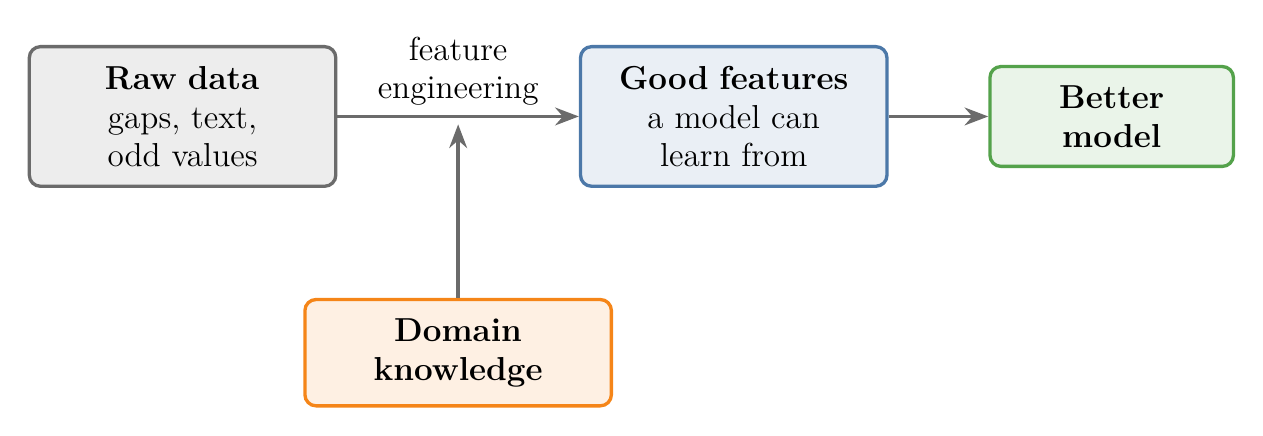
\begin{tikzpicture}[every node/.append style={font=\sffamily\large}]
\tikzset{note/.style={font=\sffamily\large, text=cgrey, align=center}}
  \node[box=cgrey, text width=3.4cm] (r) at (0,0) {\textbf{Raw data}\\gaps, text,\\odd values};
  \node[box=cblue, text width=3.4cm] (f) at (7.0,0) {\textbf{Good features}\\a model can\\learn from};
  \node[box=cgreen, text width=2.6cm] (m) at (11.8,0) {\textbf{Better}\\\textbf{model}};
  \draw[arrow] (r) -- node[above, align=center] {feature\\engineering} (f);
  \draw[arrow] (f) -- (m);
  \node[box=corange, text width=3.4cm] (d) at (3.5,-3.0) {\textbf{Domain}\\\textbf{knowledge}};
  \draw[arrow] (d) -- (3.5,-0.1);
\end{tikzpicture}
\end{document}
